\documentclass{article}
\usepackage[UTF8]{ctex}
\usepackage{amsmath,mathtools,geometry,pgfplots,float,mathrsfs,caption,enumerate}
\pgfplotsset{compat=1.15}
\usetikzlibrary{arrows}
\geometry{scale=0.7}

\title{每日一题(17.1)}
\author{\kaishu 门宇翎}
\date{2022年5月17日}

\begin{document}
\maketitle
\begin{enumerate}
	\renewcommand{\labelenumi}{\textbf{\theenumi. }}
	\item 已知$BD$, $CE$是$\triangle ABC$的高, $P$在$BD$延长线上, $BP=AC$, $Q$在$CE$上, $CQ=AB$. 求证:
	\begin{enumerate}[(1) ]
		\item$AP=AQ$;
		\item$AP\perp AQ$.
	\end{enumerate}
	\rightline{\kaishu (1996年河南省初中竞赛题)}
	\begin{figure}[H]
		\flushright
		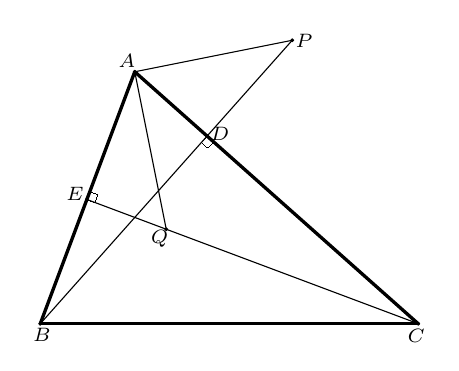
\begin{tikzpicture}[line cap=round,line join=round,>=triangle 45,x=0.8cm,y=0.8cm]
			\clip(-0.2,-0.3) rectangle (6.2,4.7);
			\draw[line width=0.pt] (0.8653884643461892,1.925479325870179) -- (0.9125118782020375,2.0511417628191078) -- (0.7868494412531086,2.098265176674956) -- (0.7397260273972602,1.9726027397260273) -- cycle; 
			\draw[line width=0.pt] (2.5591132246033004,2.879002377678713) -- (2.6594211917521737,2.789839740213048) -- (2.748583829217839,2.8901477073619213) -- (2.6482758620689655,2.9793103448275864) -- cycle; 
			\draw [line width=1.2pt] (1.5,4.)-- (0.,0.);
			\draw [line width=1.2pt] (0.,0.)-- (6.,0.);
			\draw [line width=1.2pt] (6.,0.)-- (1.5,4.);
			\draw [line width=0.4pt] (0.,0.)-- (2.6482758620689655,2.9793103448275864);
			\draw [line width=0.4pt] (6.,0.)-- (0.7397260273972602,1.9726027397260273);
			\draw [line width=0.4pt] (1.5,4.)-- (4.,4.5);
			\draw [line width=0.4pt] (2.,1.5)-- (1.5,4.);
			\draw [line width=0.4pt] (2.6482758620689655,2.9793103448275864)-- (4.,4.5);
			\begin{scriptsize}
				\draw [fill=black] (1.5,4.) circle (0.5pt);
				\draw[color=black] (1.3742064745192557,4.165315036775931) node {$A$};
				\draw [fill=black] (0.,0.) circle (0.5pt);
				\draw[color=black] (0.02663978452729976,-0.17473542958313712) node {$B$};
				\draw [fill=black] (6.,0.) circle (0.5pt);
				\draw[color=black] (5.967321108012965,-0.1873886379398691) node {$C$};
				\draw [fill=black] (2.6482758620689655,2.9793103448275864) circle (0.5pt);
				\draw[color=black] (2.854631852256898,3.0075464721349547) node {$D$};
				\draw [fill=black] (0.7397260273972602,1.9726027397260273) circle (0.5pt);
				\draw[color=black] (0.551747931331677,2.064882449558423) node {$E$};
				\draw [fill=black] (4.,4.5) circle (0.5pt);
				\draw[color=black] (4.189545333892121,4.494298454050963) node {$P$};
				\draw [fill=black] (2.,1.5) circle (0.5pt);
				\draw[color=black] (1.8929880171452669,1.356302781581432) node {$Q$};
			\end{scriptsize}
		\end{tikzpicture}
	\end{figure}
	%---%
	\item 如图, 在$\triangle ABC$中, $AB=AC$, $D$为底边$AC$上的一点, $E$为线段$AD$上的一点, 且$\angle BED=2\angle CED=\angle BAC$, 求证: $BD=2CD$.({\kaishu 1996年全国初中联赛题})
	\begin{figure}[H]
		\flushright
		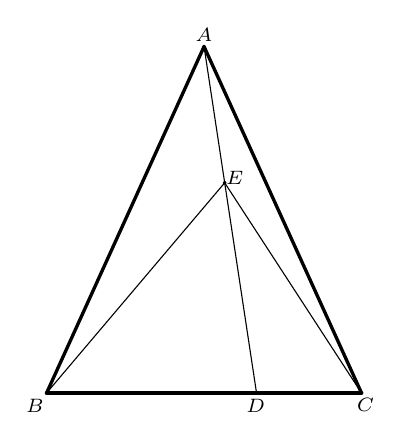
\begin{tikzpicture}[line cap=round,line join=round,>=triangle 45,x=0.8cm,y=0.8cm]
			\clip(-0.3,-0.4) rectangle (5.2,5.8);
			\draw [line width=1.2pt] (0.,0.)-- (5.,0.);
			\draw [line width=1.2pt] (0.,0.)-- (2.5,5.5);
			\draw [line width=1.2pt] (2.5,5.5)-- (5.,0.);
			\draw [line width=0.4pt] (3.333333333333334,0.)-- (2.5,5.5);
			\draw [line width=0.4pt] (2.827648114901257,3.3375224416517053)-- (0.,0.);
			\draw [line width=0.4pt] (2.827648114901257,3.3375224416517053)-- (5.,0.);
			\begin{scriptsize}
				\draw [fill=black] (0.,0.) circle (0.5pt);
				\draw[color=black] (-0.18298115521073746,-0.20102656049055967) node {$B$};
				\draw [fill=black] (5.,0.) circle (0.5pt);
				\draw[color=black] (5.063491079520078,-0.19313712855863363) node {$C$};
				\draw [fill=black] (2.5,5.5) circle (0.5pt);
				\draw[color=black] (2.4994257016441157,5.692379092658202) node {$A$};
				\draw [fill=black] (3.333333333333334,0.) circle (0.5pt);
				\draw[color=black] (3.3199266225644237,-0.2089159924224857) node {$D$};
				\draw [fill=black] (2.827648114901257,3.3375224416517053) circle (0.5pt);
				\draw[color=black] (2.986007866308492,3.4202226962634983) node {$E$};
			\end{scriptsize}
		\end{tikzpicture}
	\end{figure}
\end{enumerate}
\end{document}
